\documentclass[a4paper]{article}
\usepackage[T1]{fontenc}			% \chapter package
\usepackage[english]{babel}
\usepackage[english]{isodate}  		% date format
\usepackage{graphicx}				% manage images
\usepackage{amsfonts}
\usepackage{booktabs}				% high quality tables
\usepackage{amsmath}				% math package
\usepackage{amssymb}				% another math package (e.g. \nexists)
\usepackage{bm}                     % bold math symbols
\usepackage{mathtools}				% emphasize equations
\usepackage{stmaryrd} 				% '\llbracket' and '\rrbracket'
\usepackage{amsthm}					% better theorems
\usepackage{enumitem}				% manage list
\usepackage{pifont}					% nice itemize
\usepackage{cancel}					% cancel math equations
\usepackage{caption}				% custom caption
\usepackage[]{mdframed}				% box text
\usepackage{multirow}				% more lines in a table
\usepackage{textcomp, gensymb}		% degree symbol
\usepackage[x11names]{xcolor}		% RGB color
\usepackage{tcolorbox}				% colorful box
\usepackage{multicol}				% more rows in a table (used for the lists)
\usepackage{listings}
\usepackage{url}
\usepackage{qrcode}
\usepackage{fontawesome5}
\usepackage{ragged2e}
\usepackage{cite}                   % references
\usepackage{imakeidx}               % index
\makeindex[program=makeindex, columns=2,
           title=Index, 
           intoc,
           options={-s index-style.ist}]


\definecolor{codegreen}{rgb}{0,0.6,0}
\definecolor{codegray}{rgb}{0.5,0.5,0.5}
\definecolor{codepurple}{rgb}{0.58,0,0.82}
\definecolor{backcolour}{rgb}{0.95,0.95,0.92}
\lstdefinestyle{mystyle}{
    backgroundcolor=\color{backcolour},   
    commentstyle=\color{codegreen},
    keywordstyle=\color{magenta},
    numberstyle=\tiny\color{codegray},
    stringstyle=\color{codepurple},
    basicstyle=\ttfamily\footnotesize,
    breakatwhitespace=false,         
    breaklines=true,                 
    captionpos=b,                    
    keepspaces=true,                 
    numbers=left,                    
    numbersep=5pt,                  
    showspaces=false,                
    showstringspaces=false,
    showtabs=false,                  
    tabsize=2
}
\lstset{style=mystyle}


% draw a frame around given text
\newcommand{\framedtext}[1]{%
	\par%
	\noindent\fbox{%
		\parbox{\dimexpr\linewidth-2\fboxsep-2\fboxrule}{#1}%
	}%
}


% table of content links
\usepackage{xcolor}
\usepackage[linkcolor=black, citecolor=blue, urlcolor=cyan]{hyperref} % hypertexnames=false
\hypersetup{
	colorlinks=true
}


\newtheorem{theorem}{\textcolor{Red3}{\underline{Theorem}}}
\renewcommand{\qedsymbol}{QED}
\newcommand{\dquotes}[1]{``#1''}
\newcommand{\longline}{\noindent\rule{\textwidth}{0.4pt}}
\newcommand{\circledtext}[1]{\raisebox{.5pt}{\textcircled{\raisebox{-.9pt}{#1}}}}
\newcommand{\definition}[1]{\textcolor{Red3}{\textbf{#1}}\index{#1}}
\newcommand{\example}[1]{\textcolor{Green4}{\textbf{#1}}}
\newcommand{\highspace}{\vspace{1.2em}\noindent}


\begin{document}
    \newcounter{definition}[section]
    \newcounter{example}[section]
    
    \newtcolorbox[use counter = definition]{definitionbox}{%
        colback=red!5!white,
        colframe=red!75!black,
        fonttitle=\bfseries,
        title=Definition \thetcbcounter %
    }
    
    \newtcolorbox[use counter = example]{examplebox}{%
        colback=Green4!5!white,
        colframe=Green4!75!black,
        fonttitle=\bfseries,
        title=Example \thetcbcounter %
    }

    \author{260236}
	\title{Computing Infrastructures - Notes}
	\date{\printdayoff\today}
	\maketitle

	\newpage

    \section*{Preface}

    Every theory section in these notes has been taken from two sources:
    \begin{itemize}
        \item The Datacenter as a Computer: Designing Warehouse-Scale Machines, Third Edition.\cite{barroso2022datacenter}

        \item Quantitative System Performance: Computer System Analysis Using Queueing Network Models.\cite{lazowska1984quantitative}
    \end{itemize}
    About:
    \begin{itemize}
        \item[\faIcon{github}] \href{https://github.com/AndreVale69/HPC-E-PoliMI-university-notes}{GitHub repository}
    \end{itemize}
    
    \newpage
	
	\tableofcontents

    \newpage

    \section{Hardware Infrastructures}

    \subsection{System-level}

    \subsubsection{Computing Infrastructures and Data Center Architectures}

    There's no single definition of a Data Center, but it can be summarized as follows.
    
    \begin{definitionbox}\label{Data Center definition}
        \definition{Data Center}s are buildings where multiple servers and communication gear are co-located because of their common environmental requirements and physical security needs, and for ease of maintenance.\cite{barroso2022datacenter}
    \end{definitionbox}

    \begin{definitionbox}
        A \definition{Computing Infrastructure} (or IT Infrastructure) is a technological infrastructure that provides hardware and software for computation to other systems and services.
    \end{definitionbox}
    A number of computing infrastructures exist:
    \begin{itemize}
        \item \textbf{Cloud} offers virtualized computing, storage and network resources with highly-elastic capacity.
        
        
        \item \textbf{Edge Servers} are on-premises hardware resources that perform more compute-intensive data processing.
        
        In other words, an edge server is a piece of hardware that performs data computation at the end (or \dquotes{edge}) of a network. Like a regular server, an edge server can provide compute, networking, and storage functions.\footnote{More info \href{https://phoenixnap.com/blog/edge-server}{here}.}

        
        \item \textbf{IoT} and \textbf{AI-enabled Edge Sensors} are hardware devices where the data acquisition and partial processing can be performed at the edge of the network.
    \end{itemize}

    \newpage

    \begin{figure}[!htp]
        \centering
        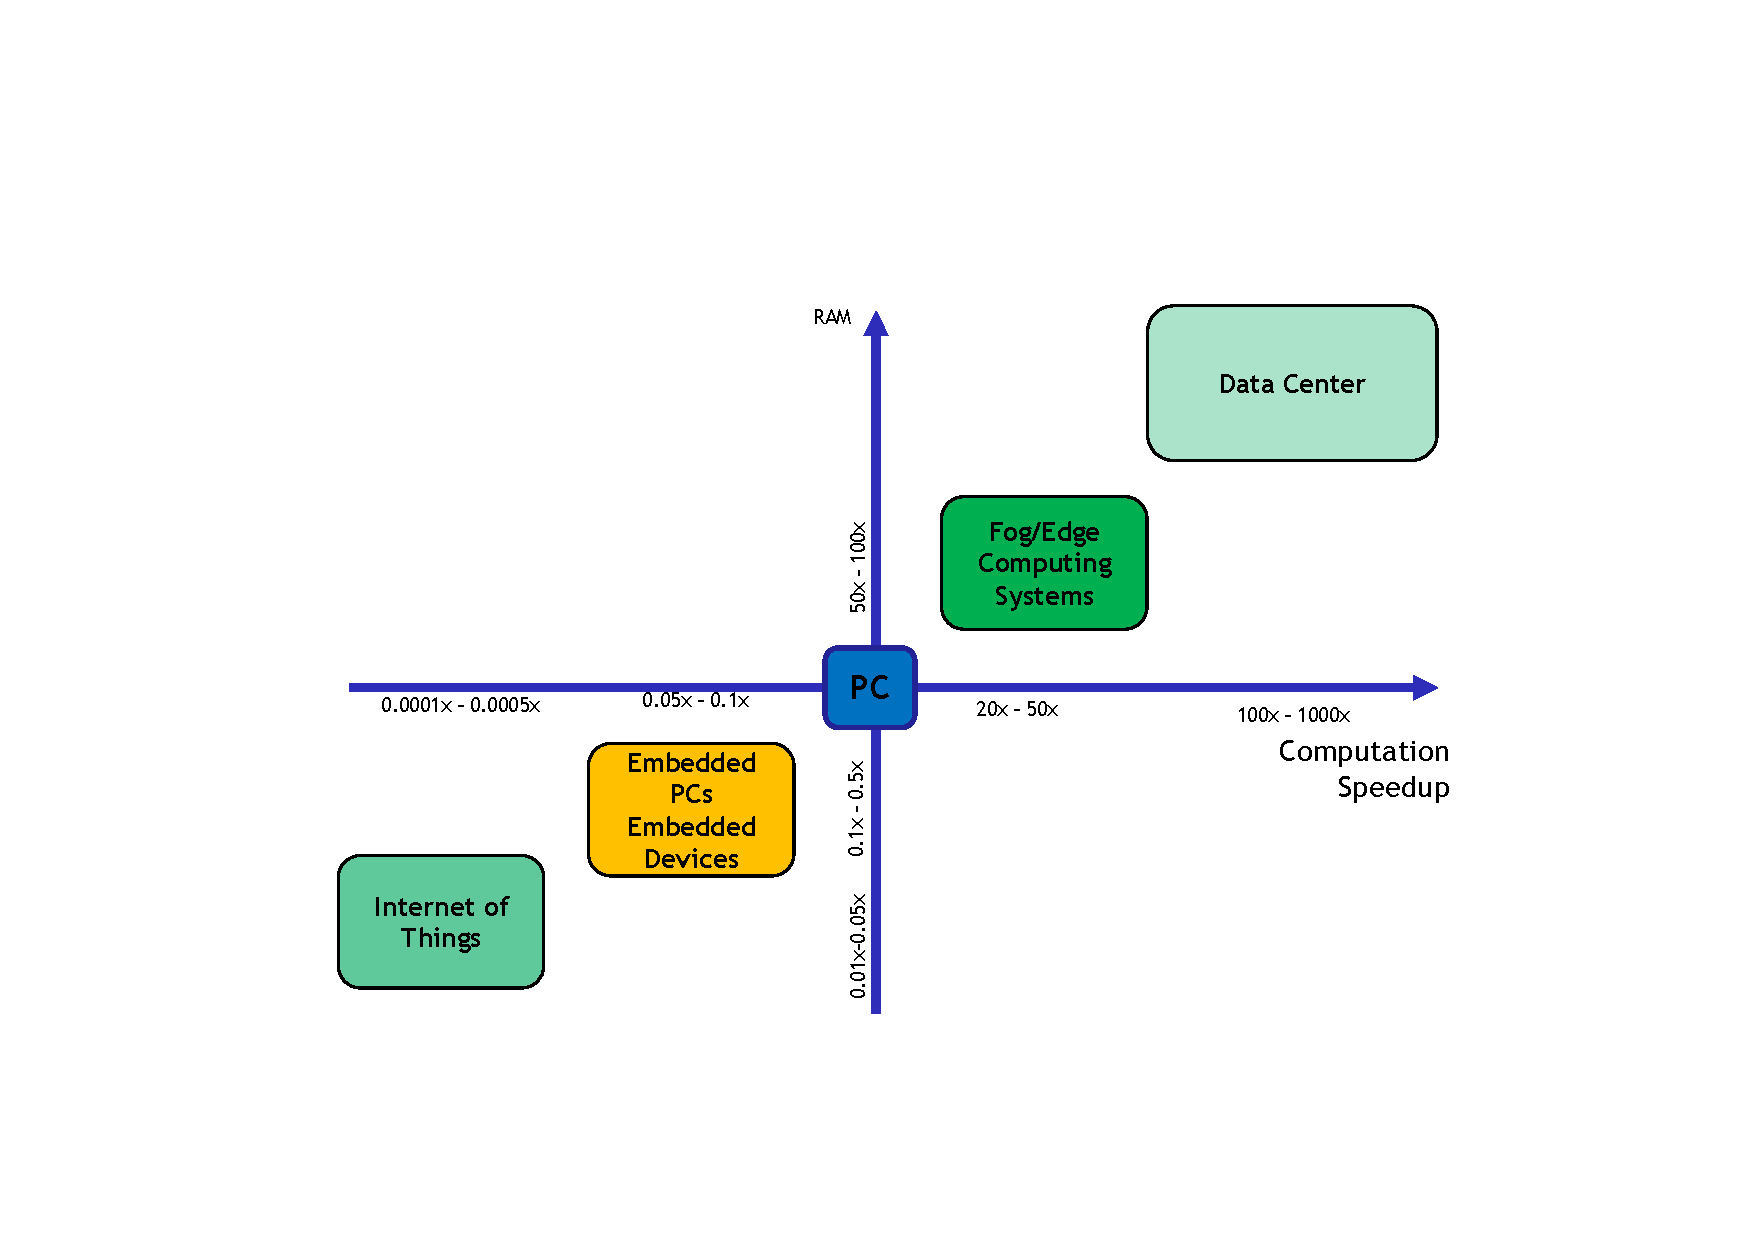
\includegraphics[width=\textwidth]{img/example-computing-infrastructure-1.pdf}
        \caption{An \example{example} of Computing Infrastructures.\cite{computing-infrastructures-slides}}
    \end{figure}

    \noindent
    The \definition{Computing Continuum}, a novel paradigm that extends beyond the current silos of cloud and edge computing, can enable the seamless and dynamic deployment of applications across diverse infrastructures.\cite{marino2023computing}

    \begin{figure}[!htp]
        \centering
        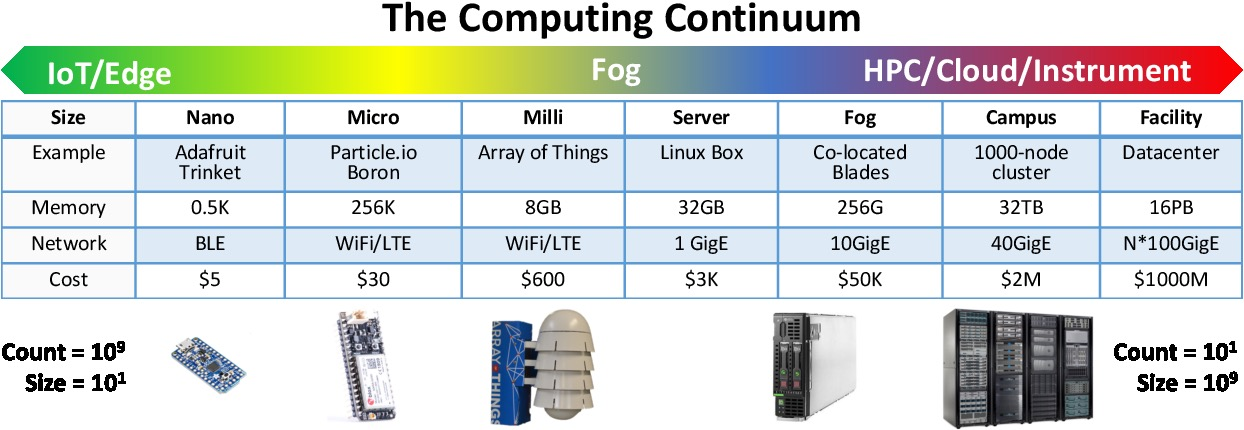
\includegraphics[width=\textwidth]{img/computing-continuum-1.png}
        \caption{The Computing Continuum.\cite{computing-infrastructures-slides}}
    \end{figure}

    \noindent
    In the following pages, we analyze the computing infrastructures mentioned in the previous example.

    \newpage

    \begin{center}
        \large
        \textcolor{Red3}{\textbf{Data Centers}}
    \end{center}
    
    \noindent
    The definition of a Data Centers can be found on page \pageref{Data Center definition}.

    \begin{flushleft}
        \textcolor{Green3}{\faIcon{check} \textbf{Data Centers Advantages}}
    \end{flushleft}
    \begin{itemize}
        \item \textbf{Lower IT costs}.
        \item \textbf{High Performance}.
        \item \textbf{Instant software updates}.
        \item \textbf{\dquotes{Unlimited} storage capacity}.
        \item \textbf{Increased data reliability}.
        \item \textbf{Universal data access}.
        \item \textbf{Device Independence}.
    \end{itemize}

    \begin{flushleft}
        \textcolor{Red2}{\faIcon{thumbs-down} \textbf{Data Centers Disadvantages}}
    \end{flushleft}
    \begin{itemize}
        \item \textbf{Require a constant internet connection}.
        \item \textbf{Do not work well with low-speed connections}.
        \item \textbf{Hardware Features might be limited}.
        \item \textbf{Privacy and security issues}.
        \item \textbf{High power Consumption}.
        \item \textbf{\underline{Latency in taking decision}}.
    \end{itemize}

    \newpage

    \begin{center}
        \large
        \textcolor{Red3}{\textbf{Internet-of-Things (IoT)}}
    \end{center}

    \noindent
    An \definition{Internet of Things (IoT)} \textbf{device is any everyday object embedded with sensors, software, and internet connectivity}.

    \highspace
    This allows to collect and exchange data with other devices and systems, typically over the internet, with limited need of process and store data.

    \highspace
    Some \example{examples} are \href{https://www.arduino.cc/}{Arduino}, \href{https://www.st.com/en/microcontrollers-microprocessors/stm32-32-bit-arm-cortex-mcus.html}{STM32}, \href{https://en.wikipedia.org/wiki/ESP32}{ESP32}, \href{https://docs.particle.io/argon/}{Particle Argon}.

    \begin{flushleft}
        \textcolor{Green3}{\faIcon{check} \textbf{Internet-of-Things Advantages}}
    \end{flushleft}
    \begin{itemize}
        \item \textbf{Highly Pervasive}.
        \item \textbf{Wireless connection}.
        \item \textbf{Battery Powered}.
        \item \textbf{Low costs}.
        \item \textbf{Sensing and actuating}.
    \end{itemize}

    \begin{flushleft}
        \textcolor{Red2}{\faIcon{thumbs-down} \textbf{Internet-of-Things Disadvantages}}
    \end{flushleft}
    \begin{itemize}
        \item \textbf{Low computing ability}.
        \item \textbf{Constraints on energy}.
        \item \textbf{Constraints on memory (RAM/FLASH)}.
        \item \textbf{Difficulties in programming}.
    \end{itemize}

    \longline

    \begin{center}
        \large
        \textcolor{Red3}{\textbf{Embedded (System) PCs}}
    \end{center}

    \noindent
    An \definition{Embedded System} is a computer system, a combination of a computer processor, computer memory, and input/output peripheral devices, that has a dedicated function within a larger mechanical or electronic system.

    \highspace
    A few \example{examples}: \href{https://www.hardkernel.com/}{Odroid}, \href{https://www.raspberrypi.com/}{Raspberry}, \href{https://developer.nvidia.com/embedded/jetson-nano}{jetson nano}, \href{https://www.coral.ai/}{Google Coral}.

    \begin{flushleft}
        \textcolor{Green3}{\faIcon{check} \textbf{Embedded System Advantages}}
    \end{flushleft}
    \begin{itemize}
        \item \textbf{Persuasive computing}.
        \item \textbf{High performance unit}.
        \item \textbf{Availability of development boards}.
        \item \textbf{Programmed as PC}.
        \item \textbf{Large community}.
    \end{itemize}

    \begin{flushleft}
        \textcolor{Red2}{\faIcon{thumbs-down} \textbf{Embedded System Disadvantages}}
    \end{flushleft}
    \begin{itemize}
        \item \textbf{Pretty high power consumption}.
        \item \textbf{(Some) Hardware design has to be done}.
    \end{itemize}

    \newpage

    \begin{center}
        \large
        \textcolor{Red3}{\textbf{Edge/Fog Computing Systems}}
    \end{center}

    \noindent
    The key \textbf{difference} between \definition{Fog Computing} and \definition{Edge Computing} is associated with the location \textbf{where the data is processed}:
    \begin{itemize}
        \item In \textbf{edge computing}, the data is processed closest to the sensors.

        \item In \textbf{fog computing}, the computing is moved to processors linked to a local area network (IoT gateway).
    \end{itemize}
    Edge computing places the intelligence in the connected devices themselves, whereas, fog computing puts in the local area network.

    \newpage

    \bibliography{bibtex}{}
    \bibliographystyle{plain}

    \newpage

    \printindex
\end{document}